\documentclass[class=article]{standalone}

%\documentclass[12pt]{article}
%
%\usepackage{../preambolo}
%
%\usepackage[
%style=numeric,
%natbib=true,
%backend=biber,
%sorting=ynt,
%maxbibnames=99
%]{biblatex}
%\addbibresource{fisicaBib.bib}

\begin{document}	
	\section{Fisica della Bicicletta}
	Per meglio comprendere i capitoli seguenti andremo ora ad analizzare i principali fenomeni fisici che influenzano la bicicletta durante il moto.
	
	\begin{center}
		\begin{figure}[h!]
			\centering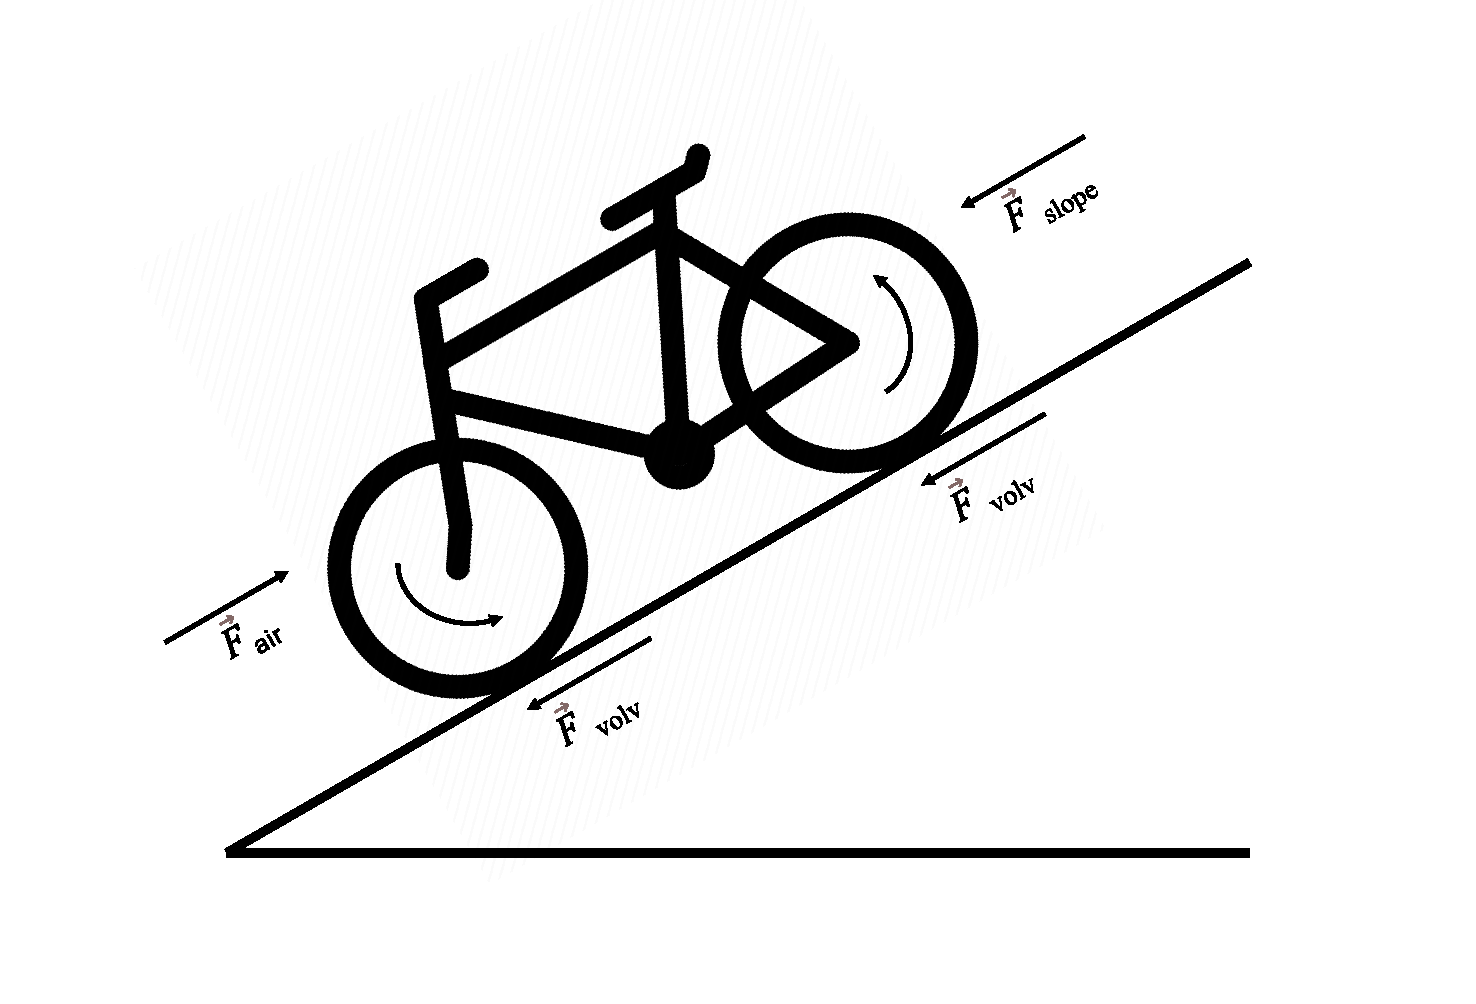
\includegraphics[width=.8\textwidth]{img/potenze}
			\caption[]{Forze resistenti applicate a una bicicletta che va in discesa.}
			\label{fig:potenze}
		\end{figure}
	\end{center}
	
	\subsection{Dinamica Longitudinale}
	La dinamica longitudinale riguarda tutte quelle forze che consentono l'avanzamento della bicicletta. Affinché questa acceleri le deve essere applicata una forza
	\[\vec{F}=m_{sys}\cdot a_{bike}\]
	dove \(a_{bike}\) è l'accelerazione della bicicletta e \(m_{sys}\) è la massa del sistema ovvero la somma della massa del ciclista \(M_{ciclista}\) e quella della bicicletta \(m_{bike}\).
	\[m_{sys}=m_{bike}+M_{ciclista}\]
	
	Possiamo quindi scomporre il vettore \(\vec{F}\) nelle sue componenti \(\vec{F}_{P}\) e \(\vec{F}_{R}\)
	
	\[\vec{F}_{P}-\vec{F}_{R}=m_{sys}\cdot a_{bike}\]
	dove \(\vec{F}_{P}\) è la forza propulsiva, ovvero la forza che tende a far accelerare la bicicletta, mentre \(\vec{F}_{R}\) è la forza resistente, cioè la forza che si oppone al movimento della stessa.
	
	Abbiamo quindi che:
	\begin{itemize}
		\item se \(\vec{F}_{P}>\vec{F}_{R} \rightarrow a_{sys}>0\) la bicicletta accelera
		\item se \(\vec{F}_{P}<\vec{F}_{R} \rightarrow a_{sys}<0\) la bicicletta decelera
		\item se \(\vec{F}_{P}=\vec{F}_{R} \rightarrow a_{sys}=0\) la bicicletta si muove a velocità costante.
	\end{itemize}
	
	Per semplificare le cose consideriamo di trovarci in quest'ultimo caso, supponiamo quindi che il ciclista stia avanzando mantenendo la velocità della bicicletta \(v_{bike}\) costante.
		
	\[a_{bike}=0 \rightarrow \vec{F}_{P}=\vec{F}_{R}\]
	
	Moltiplicando ora \(\vec{F}_{R}\) per \(v_{bike}\) possiamo convertire la forza resistente in potenza resistente
	
	\[P_{P}=P_{R}=\vec{F}_{R}\cdot v_{bike}\]
	dove \(P_{P}\) è la potenza propulsiva che è pari a
	
	\[P_{P}=P_{in}\cdot\eta\]
	con \(\eta\) il rapporto di trasmissione tra pedali e ruota e \(P_{in}\) la potenza in ingresso al sistema
	
	\[P_{in}=\vec{F}_{in}\cdot cos(\theta)\cdot l_{crank}\cdot\omega_{crank}\]
	dove \(l_{crank}\) e \(\omega_{crank}\) sono, rispettivamente, la lunghezza e la velocità angolare della pedivella e \(\theta\) è angolo compreso tra la direzione del vettore \(\vec{F}_{in}\) (la forza che il ciclista applica sui pedali) e l'asse perpendicolare alla pedivella. Abbiamo quindi che, in funzione della posizione in cui si trova la pedivella, il ciclista sarà in grado di imprimere una forza maggiore o minore alla bicicletta. In particolare la forza propulsiva risulta massima quando le pedivelle sono parallele al terreno e minima quando sono perpendicolari allo stesso. L'accelerazione della bicicletta risulta quindi oscillante.
	
	Applicando quanto scritto nei passaggi precedenti otteniamo
	
	\[\vec{F}_{in}\cdot cos(\theta)\cdot l_{crank}\cdot \omega_{crank}\cdot\eta=\vec{F}_{R}\cdot v_{bike}\]
	
	Passiamo ora alla forza resistente \(\vec{F}_{R}\). Come detto questa è la forza che si oppone al movimento della bicicletta ed è composta dalle seguenti componenti
	
	\[\vec{F}_{R}=\vec{F}_{air}+\vec{F}_{volv}-\vec{F}_{slope}\]
	
	dove	
	\begin{itemize}
		\item \(\vec{F}_{air}\) è la forza di attrito dell'aria
		\[\vec{F}_{air}=\frac{1}{2}\rho_{air}\cdot C_{d}\cdot A\cdot v_{air}^2\]
		dove \(\rho_{air}\) è la densità dell'aria, \(C_{d}\) è il coefficiente d'attrito, \(A\) è l'area frontale del ciclista e della bicicletta e \(v_{air}\) è la velocità dell'aria rispetto alla bicicletta ed è quindi composta dalla velocità del ciclista \(v_{bike}\) e dalla velocità del vento \(v_{wind}\) 
		\[v_{air}=v_{bike}+v_{wind}\]
		\[\vec{F}_{air}=\frac{1}{2}\rho_{air}\cdot C_{d}\cdot A\cdot (v_{bike}+v_{wind})^2\]
		
		\item \(\vec{F}_{volv}\) è la forza di attrito volvente
		\[\vec{F}_{volv}=m_{sys}\cdot g\cdot \mu_{v}\cdot cos(\alpha)\]
		dove \(\mu_{v}\) è il coefficiente d'attrito volvente, \(g\) è la forza di gravità e \(\alpha\) è l'inclinazione della superficie sulla quale sta andando la bicicletta. Questa forza è quindi massima quando la bicicletta si muove su un piano orizzontale.
		
		\item \(\vec{F}_{slope}\) è la forza che la bicicletta subisce a causa della gravità
		\[\vec{F}_{slope}=m_{sys}\cdot g\cdot sin(\alpha)\]
		e si oppone al movimento quando la bicicletta si muove in salita (\(\alpha > 0\)) e, al contrario, favorisce il movimento quando la bicicletta si muove in discesa (\(\alpha < 0\)).
	\end{itemize}
	
	Per quanto detto precedentemente otteniamo
	\[\vec{F}_{in}\cdot cos(\theta)\cdot l_{crank}\cdot \omega_{crank}\cdot\eta=(\vec{F}_{air}+\vec{F}_{volv}-\vec{F}_{slope})\cdot v_{bike}\]
	
	\[\vec{F}_{in}\cdot cos(\theta)\cdot l_{crank}\cdot \omega_{crank}\cdot\eta=\]
	\[=(\frac{1}{2}\rho_{air}\cdot C_{d}\cdot A\cdot (v_{bike}+v_{wind})^2+m_{sys}\cdot g\cdot \mu_{v}\cdot cos(\alpha)-m_{sys}\cdot g\cdot sin(\alpha))\cdot v_{bike}\]
	che ci mostra come, all'aumentare della velocità, al ciclista sia richiesto di generare una maggior potenza. Inoltre, nel caso in cui il ciclista volesse accelerare entrerebbe in gioco anche l'inerzia, che dipende dalla massa del sistema e dal momento d'inerzia della ruota, che si andrebbe a sommare alle altre forze resistenti.
	Da quanto detto finora ne segue che, visto che per poter accelerare è necessario vincere le forze resistenti, tanto più la velocità della bicicletta è elevata tanto più è difficile accelerare.
			
	\subsection{Dinamica Laterale}
	La dinamica laterale si occupa delle forze e dei momenti che agiscono sulla bicicletta durante i movimenti laterali, in particolare le curve.
	
	Le forze che entrano in gioco durante le curve sono:
	\begin{itemize}
		\item forza di attrito laterale
		\item forza centripeta
		\item forza centrifuga
	\end{itemize}
	
	La forza di attrito laterale è la forza di attrito tra gli pneumatici e il terreno ed è ciò che consente alla bicicletta di curvare.
	
	La forza centripeta	è una forza che agisce dall'esterno verso l'interno e che consente di mantenere la traiettoria durante la curva. È data da
	\[\vec{F}_{centripeta}=m_{sys}\cdot\frac{v_{bike}^2}{R}\]
	dove \(R\) è il raggio della curva, ovvero la distanza tra la bicicletta e il centro di istantanea rotazione.
	
	La forza centrifuga \(\vec{F}_{c}\), infine, è una forza che agisce dall'interno verso l'esterno di modulo pari alla forza centripeta ma di verso opposto.
	In particolare la forza centrifuga è applicata al centro di massa della sistema \(ciclista + bicicletta\) e tende a far ruotare lo stesso attorno all'asse che congiunge i punti di contatto delle due ruote con il terreno, generando un momento \(\vec{M}_{c}\).
	\[\vec{F}_{c}=m_{sys}\cdot\frac{v_{bike}^2}{R}\]
	\[\vec{M}_{c}=\vec{F}_{c\perp}\cdot h=\vec{F}_{c}\cdot cos(\phi_{roll})\cdot l=m_{sys}\cdot\frac{v_{bike}^2}{R}\cdot cos(\phi_{roll})\cdot l\]
	dove \(\phi_{roll}\) è l'angolo di rollio, ovvero la rotazione della bicicletta attorno all'asse longitudinale e \(l\) è la distanza minima tra il centro di massa del sistema e l'asse che congiunge i punti di contatto delle due ruote con il terreno.
	
	Per bilanciare questo momento, ed evitare di cadere, il ciclista è costretto a inclinarsi, in modo che la forza di gravità generi un secondo momento \(\vec{M}_{g}\)
		\[\vec{F}_{g}=m_{sys}\cdot g\]
	\[\vec{M}_{g}=m_{sys}\cdot g \cdot sin(\phi_{roll})\cdot l\]
	che vada a compensare \(\vec{M}_{c}\).	

	\[\vec{M}_{c}=\vec{M}_{g}\]
	\[m_{sys}\cdot\frac{v_{bike}^2}{R}\cdot cos(\phi_{roll})\cdot l=m_{sys}\cdot g \cdot sin(\phi_{roll})\cdot l\]
	
	Dall'uguaglianza precedente è possibile ricavare l'angolo alla quale i due momenti si equivalgono, ovvero di quanto il ciclista deve inclinare la bicicletta per evitare di cadere durante la curva.
	
	\[tg(\phi_{roll})=\frac{v_{bike}^2}{R\cdot g} \rightarrow \phi_{roll}=arctg\left(\frac{v_{bike}^2}{R\cdot g}\right)\]
	
	Infine, è importante considerare che, durante la pedalata, la forza che il ciclista applica sul pedale genera un momento che tende a far ruotare la bicicletta attorno all'asse longitudinale. Avremo quindi che, durante la corsa, la bicicletta oscillerà a destra e a sinistra in base a quale dei due pedali il ciclista sta impiegando per pedalare in quel momento.
	
%	\newpage
%	\printbibliography[title={Bibliografia}]
	
	
\end{document}